\documentclass{article}

\usepackage{graphicx}

\begin{document}
\title{Homework 15}
\date{}
\maketitle

% 1. Fall 2009 Final, #4
% 2. Fall 2010 Final, #5
% 3. Textbook 4.3.1 and 4.4.1

\paragraph{\Large 1. Spring 2008 Final Questions 2a and 2b}\mbox{}\\
Run \textit{Dijkstra’s algorithm} on the weighted digraph below, starting at vertex $A$.\\
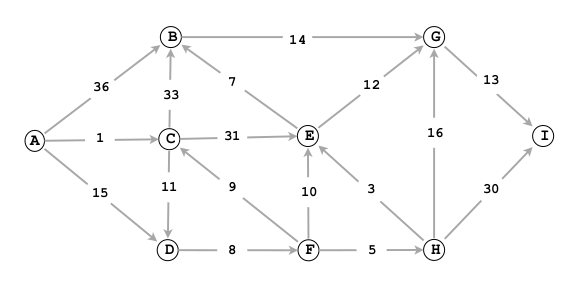
\includegraphics[]{fin-f09-4.png}\\
\begin{enumerate}
\renewcommand{\theenumi}{\Alph{enumi}}
	\item List the vertices in the order in which the vertices are dequeued (for the first time) from the priority queue and give the length of the shortest path from $A$.\\
	
	vertex: A C D F H E B G I\\

	distance: 0 1 12 20 25 28 34 40 43

	\item Draw the edges in the shortest path tree with thick lines in the figure above.\\

	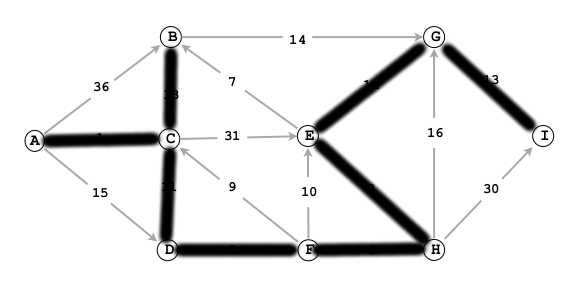
\includegraphics[]{fin-f09-4b.png}

\end{enumerate}


\paragraph{\Large 2. Fall 2010 Final Question 5}\mbox{}\\
Run the eager version of Dijkstra’s algorithm on the following edge-weighted digraph, starting from vertex 0.\\
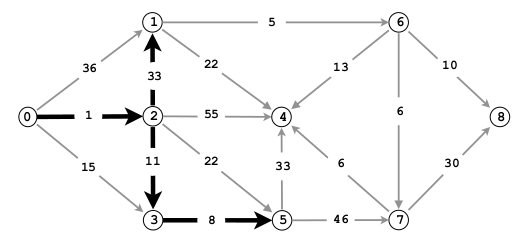
\includegraphics[]{fin-f10-5.png}
\begin{enumerate}
\renewcommand{\theenumi}{\Alph{enumi}}
	\item Complete the table of edgeTo[ ] and distTo[ ] values immediately after the first 5 vertices (0, 2, 3, 5, and 1) have been deleted from the priority queue and relaxed.\\

	\begin{tabular}{c l c}
	v & edgeTo[ ] & distTo[ ]\\
	0 & \hspace{2mm}- & 0.0\\
	1 & $2 \rightarrow 1$ 33.0 & 34.0\\
	2 & $0 \rightarrow 2$ 1.0 & 1.0\\
	3 & $2 \rightarrow 3$ 11.0 & 12\\
	4 & $5 \rightarrow 4$ 33.0 & 53.0\\
	5 & $3 \rightarrow 5$ 8.0 & 20.0\\
	6 & $1 \rightarrow 6$ 5.0 & 39.0\\
	7 & $5 \rightarrow 7$ 46.0 & 66.0\\
	8 & \hspace{2mm}- & -
	\end{tabular}

	\item Complete the table of edgeTo[ ] and distTo[ ] values immediately after the 6 th vertexhas been deleted from the priority queue and relaxed. Circle those values that changed from A.\\

	\begin{tabular}{c l c}
	v & edgeTo[ ] & distTo[ ]\\
	0 & \hspace{2mm}- & 0.0\\
	1 & $2 \rightarrow 1$ 33.0 & 34.0\\
	2 & $0 \rightarrow 2$ 1.0 & 1.0\\
	3 & $2 \rightarrow 3$ 11.0 & 12\\
	\textbf{4} & $\mathbf{6 \rightarrow 4}$ \textbf{13.0} & \textbf{52.0}\\
	5 & $3 \rightarrow 5$ 8.0 & 20.0\\
	6 & $1 \rightarrow 6$ 5.0 & 39.0\\
	\textbf{7} & $\mathbf{6 \rightarrow 7}$ \textbf{6.0} & \textbf{45.0}\\
	\textbf{8} & $\mathbf{6 \rightarrow 8}$ \textbf{10.0} & \textbf{49.0}
	\end{tabular}

\end{enumerate}

\paragraph{\Large 3. Question 4.3.1}\mbox{}\\
Prove that you can rescale the weights by adding a positive constant to all of them or by multiplying them all by a positive constant without affecting the MST.\\

Edge weights increased by a common number maintain the same differences from each other and, thus, quite obviously maintain the same MST. While multiplication by a common number does not maintain the exact edge differences, the edge ratios are preserved. Thus, any edge $E$ that was less than any other edge $E'$ must continue to be less than $E'$ when both are multiplied by a common factor.

\paragraph{\Large 4. Question 4.4.1}\mbox{}\\
True of false: Adding a constant to every edge weight does not change the solution to the single-source shortest-paths problem.\\

False. In the case of negative edge weights, a constant can affect whether a path is the shortest.

\end{document}